%%%%%%%%%%%%%%%%%%%%%%%%%%%%%%%%%%%%%%%%%%%%%%%%%%%%%%%%%%%%%%%%%%%%%%%%%%%%%%%%
%2345678901234567890123456789012345678901234567890123456789012345678901234567890
%        1         2         3         4         5         6         7         8

\documentclass[letterpaper, 10 pt, conference]{ieeeconf}  % Comment this line out if you need a4paper

%\documentclass[a4paper, 10pt, conference]{ieeeconf}      % Use this line for a4 paper

\IEEEoverridecommandlockouts                              % This command is only needed if 
                                                          % you want to use the \thanks command

\overrideIEEEmargins                                      % Needed to meet printer requirements.

%In case you encounter the following error:
%Error 1010 The PDF file may be corrupt (unable to open PDF file) OR
%Error 1000 An error occurred while parsing a contents stream. Unable to analyze the PDF file.
%This is a known problem with pdfLaTeX conversion filter. The file cannot be opened with acrobat reader
%Please use one of the alternatives below to circumvent this error by uncommenting one or the other
%\pdfobjcompresslevel=0
%\pdfminorversion=4

% See the \addtolength command later in the file to balance the column lengths
% on the last page of the document

% The following packages can be found on http:\\www.ctan.org
\usepackage{graphics} % for pdf, bitmapped graphics files
\usepackage{epsfig} % for postscript graphics files
\usepackage{mathptmx} % assumes new font selection scheme installed
\usepackage{times} % assumes new font selection scheme installed
\usepackage{amsmath} % assumes amsmath package installed
\usepackage{amssymb}  % assumes amsmath package installed
\usepackage{mathtools}
\usepackage{relsize}
\usepackage{tikz}
\graphicspath{{./Drawings/}} 
\newcommand{\notimplies}{%
	\mathrel{{\ooalign{\hidewidth$\not\phantom{=}$\hidewidth\cr$\implies$}}}}
\usepackage[margin=0.8cm]{caption}
\newcommand{\norm}[1]{\left\lVert#1\right\rVert}
\usepackage{pgfplots}
\pgfplotsset{compat=newest}
\pgfplotsset{plot coordinates/math parser=false}
\newlength\figureheight
\newlength\figurewidth 
\usepackage{adjustbox}
\usepackage{indentfirst}

\newcommand*{\CC}{%
	\textsf{C\kern-1ex C}%
}
\newcommand*{\RR}{%
	\textsf{I\kern-.3ex R}%
}
\newcommand*{\ZZ}{%
	\textsf{Z\kern-1ex Z}%
}


\newtheorem{lemma}{Lemma}
\newtheorem{theorem}{Theorem}
\newtheorem{assumption}{Assumption}
\newtheorem{proposition}{Proposition}
\usepackage{lineno,amssymb,subcaption,algpseudocode,algorithm}


\setlength{\parindent}{15pt} % Default is 15pt.
\newcommand{\AB}[1]{\textbf{\color{magenta}{[AB: #1]}}}
\newcommand{\SK}[1]{\textbf{\color{blue}{[SK: #1]}}}
\newcommand{\SKN}[1]{\textbf{\color{red}{#1}}}
\newcommand{\smallmat}[1]{\left[ \begin{smallmatrix}#1 \end{smallmatrix} \right]}

\title{\LARGE \bf
Identification of exogenous disturbance signal sets
}


\author{XYZ, A.Bemporad% <-this % stops a space
\thanks{*This work was not supported by any organization}% <-this % stops a space
\thanks{Sampath Kumar Mulagaleti and Alberto Bemporad are with
		the IMT School for Advanced Studies Lucca, Piazza San Francesco 19,
		55100 Lucca, Italy. 
		 Email: 
	   {\tt\small \{s.mulagaleti,alberto.bemporad\}@imtlucca.it}}%%
}

\bibliographystyle{ieeetr}
\begin{document}



\maketitle
\thispagestyle{empty}
\pagestyle{empty}


%%%%%%%%%%%%%%%%%%%%%%%%%%%%%%%%%%%%%%%%%%%%%%%%%%%%%%%%%%%%%%%%%%%%%%%%%%%%%%%%
\begin{abstract}

This work deals with uncertain linear models of dynamical systems, with the uncertainty modeled as an exogenous disturbance signal acting on the output. A method to identify the set within which this uncertainty lies is presented. 

\end{abstract}


%%%%%%%%%%%%%%%%%%%%%%%%%%%%%%%%%%%%%%%%%%%%%%%%%%%%%%%%%%%%%%%%%%%%%%%%%%%%%%%%
\section{Introduction}
Model predictive control schemes can be used to design controllers for systems with constraints. The schemes choose a control input by making predictions of the future evolution of the system. They use a model of the system being controlled to make these predictions. Very often, the model does not represent the system exactly, resulting in the predictions not being accurate. This can result in the system constraints being violated. To avoid this, robust model predictive control schemes have been proposed in literature. A review of the considerations to be made while developing such robust schemes can be found in \cite{10.1007/BFb0109870}. In the current work, we deal with uncertainty descriptions.  
 \\ \indent
 Uncertainty descriptions are explicit characterizations of the uncertainty present within the model. Such a characterization helps in establishing bounds on the predictions made by the model, such that the real performance of the system lies within these bounds. The robust model predictive controller scheme should ensure constraint satisfaction for all possible predictions of the system evolution within these bounds.  
 
\section{Problem Statement}
We consider a \textit{multi-input multi-output} plant, generating an output signal $y(t) \in  \RR^{n_y}$ corresponding to the input signal $y(t) \in\RR^{n_u}, t \in \ZZ^+$. We aim at synthesizing a controller that can make the output track a user-defined reference signal $r(t) \in  \RR^{n_y}$, while robustly respecting the polyhedral constraints $Hy(t) \leq h , t \in \ZZ^+$. Towards this end, we first perform an experiment to identify a model of the plant, the details of which are given in the next section. 
\section{Open-loop model identification}
An ARX model of a open-loop dynamical system is identified, which is parameterized as follows:
\begin{equation*} 
A(q^{-1})y(t)=B(q^{-1})u(t)+w(t)
\end{equation*}
For this, the dataset $D_N=\{u(k),y(k);k\in1,2,..,N\}$ obtained from open-loop experiments is utilized. Assuming the model is invertible, it is rewritten as
\begin{equation} 
y(t)=M(q^{-1})u(t)+D(q^{-1})w(t)
\label{tfmodel}
\end{equation}
where the transfer functions are $M(q^{-1})=B(q^{-1})/A(q^{-1})$ and $D(q^{-1})=1/A(q^{-1})$. Hence, the output $y(t)$ is the sum of outputs of two systems, a schematic of which is shown here:
\begin{figure}[h]
	\hspace{20pt}
	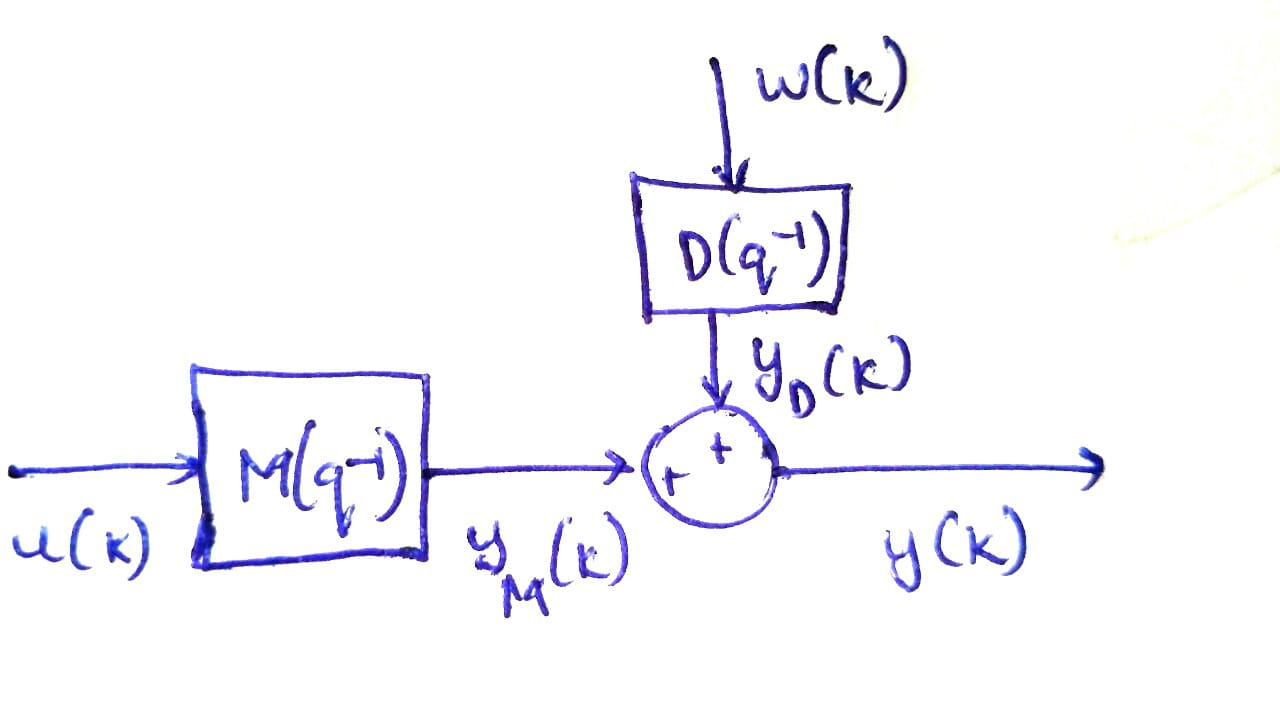
\includegraphics[scale=0.15]{schematic.jpeg}
	\caption{ARX model}
\end{figure} \\
If the dataset $D_N$ is noise-free, the part $y_D(t)$ of the output $y(t)$ that the model $M(q^{-1})$ does not capture can be attributed to model uncertainty. Hence, the uncertainty is modeled as an exogenous disturbance signal acting on the output. Robust model-based control schemes can utilize this model for controller synthesis, provided the uncertainty set the exogenous disturbance signal $w(t)$ belongs to is available. In the next section, one such control scheme is discussed. Following that, a method to obtain the set in which $w(t)$ lies is presented.
  \section{Robust controller design}
  For controller synthesis, we first
  convert the transfer function in Eq.\eqref{tfmodel} to state space form, and obtain the following equations:
  \begin{equation} 
  \begin{matrix}
  \begin{bmatrix}
  x_M(t+1) \\ x_D(t+1)
  \end{bmatrix} = 
  \begin{bmatrix}
  A_M & 0 \\ 0 & A_D
  \end{bmatrix}
  \begin{bmatrix}
  x_M(t) \\ x_D(t)
  \end{bmatrix} + 
  \begin{bmatrix}
  B_M \\ 0
  \end{bmatrix}
  u(t)+ 
  \begin{bmatrix}
  0 \\ B_D
  \end{bmatrix}
  w(t) \\ \\
  y(t) = 
  \begin{bmatrix}
  C_M & C_D
  \end{bmatrix}
  \begin{bmatrix}
  x_M(t) \\ x_D(t)
  \end{bmatrix}
  + D_Mu(t) + D_Dw(t) 
  \end{matrix}
  \label{ssmodel}
  \end{equation}
  where the states $x_M(t)$ and $x_D(t)$ belong to the system model $M$ and the disturbance model $D$ respectively. 
  In a condensed way, they are written as:
  \begin{equation}
  \begin{matrix}
    x(t+1)=Ax(t)+B_Uu(t)+B_Ww(t) \\
    y(t)=Cx(t)+D_Uu(t)+D_Ww(t) 
    \end{matrix} 
        \label{ssmodel_condensed}
    \end{equation}
    \begin{table*}[t]
    	\begin{equation}
    	\mathbb{O}_{N_P}= \begin{Bmatrix}
    	(x(t),\bar{u}):
    	\tilde{H}
    	\begin{pmatrix}
    	\begin{bmatrix}
    	CA \\ CA^2 \\ . \\ . \\ CA^{N_P}
    	\end{bmatrix}x(t) +
    	\begin{bmatrix}
    	CB_U+D_U \\ CAB_U+D_U \\ . \\ . \\ C\sum\limits_{j=0}^{N_P-1}A^{j}B_U + D_{U}
    	\end{bmatrix}\bar{u} + 
    	\begin{bmatrix}
    	CB_W & D_W & . & .  & 0 \\ CAB_W & CB_W & D_W & . & 0 \\ . \\ . \\ CA^{N_P-1}B_W & CA^{N_P-2}B_W & . & . & D_W
    	\end{bmatrix}
    	\begin{bmatrix}
    	w(t) \\ w(t+1) \\ . \\ . \\ w(t+N_P)
    	\end{bmatrix} 
    	\end{pmatrix}
    	\leq
    	\tilde{h}
    	\end{Bmatrix}
    	\label{full_ONP}
    	\end{equation}
    \end{table*}
  A robust reference governor can be designed to provide a control input $u(t)$ that makes the output $y(t)$ 
  track a reference signal $r(t)$. At each time step $t$, the controller solves the optimization problem:
  	\begin{equation}
  	\small
  	\begin{aligned}
  	\underset{\bar{u}}{\text{min}}
  	&  \hspace{20pt} \mathlarger{\sum\limits_{k=1}^{N_P}}(\hat y(t+k)-r(t+k))^2 \\
  	\text{subject to}
  	%\begin{matrix}
  	& \hspace{20pt} \hat{x}(t+k+1) = A\hat{x}(t+k) + B_U\bar{u}\\
  	& \hspace{20pt} \hat y(t+k) = C\hat{x}(t+k) + D_U\bar{u} \\
  	& \hspace{20pt} \hat{x}(t)=x(t) \\
  	& \hspace{20pt} (x(t),\bar{u}) \in \mathbb{O}_{N_P}
  	%	& \hspace{20pt} Hy_{\gamma}(t) \leq h \mbox{\AB{I think $Hy_{\gamma}(t)\leq h$ is redundant}}\\
  	%	& \hspace{20pt}  g(t+k) \in \mathbb{G}_{N_P}(\gamma(t)) \\
  	%\end{matrix}
  	\end{aligned}
  	\label{RMPC}
  	\end{equation}
  It reads the initial state $x(t)$ of the system, and calculates a constant control input $\bar{u}$ which is feasible with respect to the output admissible set $\mathbb{O}_{N_P}$ of the system Eq.\eqref{ssmodel} defined as:
  \begin{equation}
  \begin{matrix}
  \mathbb{O}_{N_P} = \{(x(t),\bar{u}):y\in \mathbb{Y}, u(t+k)=\bar{u},\forall w \in \mathbb{W}  \\ \hspace{150pt} \forall k \in \{1,2,..,N_P\} \}
  \end{matrix}
  \label{O_form}
  \end{equation}
  where $y \in \mathbb{Y}$ denotes the future output sequence $\{y(t+k)\in\mathbb{Y},k=1,..,N_P\}$
  and $w \in \mathbb{W}$ denotes the future disturbance sequence $\{w(t+k)\in\mathbb{W},k=0,..,N_P\}$.
  It is the set of initial states $x(t)$ and a constant control input $\bar{u}$ such that the future output trajectory of the system does not violate the constraints defined by $\mathbb{Y}$ for any possible bounded disturbance sequence $w\in\mathbb{W}$, within the horizon time $N_P$. 
  \\
  At any future time instant $t+k$, given the initial state $x(t)$ and a constant control input $\bar{u}$, the output $y(t+k)$ is given by:
  	\begin{equation}
  	\hspace{-30pt}
  	\begin{aligned}
  	\begin{matrix}
  	y(t+k) = CA^{k}x(t) + \bigg( C\sum\limits_{j=0}^{k-1}A^{j}B_U + D_{U} \bigg)\bar{u} + \vspace{5pt}\\  \hspace{110pt} C\sum\limits_{j=0}^{k-1}A^jB_Ww(t+k-1-j) + D_{W} w(t+k)
  	\end{matrix}
  	\end{aligned}
  	\label{elongform}
  	\end{equation}
  	It is desired to constraint the output $y(t+k)$ at a time instant $t+k$ within the polyhedral set $Hy(t+k) \leq h, h \in I\!R^{n_c}$.
  The output constraint set $\mathbb{Y}$ represents a collection of these pointwise in time polyhedron constraints, and is written as:
  \begin{equation*}
  \small
  \mathbb{Y}=\begin{Bmatrix}y:
  \begin{bmatrix}
  H & . & . & 0 \\
  . & H & . & .\\
  . & . & . & . \\
  0 & . & . & H
  \end{bmatrix}
  \begin{bmatrix}
  y(t+1) \\ . \\ . \\ y(t+N_P)
  \end{bmatrix}
  \leq \begin{bmatrix}
  h \\ . \\ . \\  h
  \end{bmatrix}
  \end{Bmatrix} = 
  \{ y: \tilde{H} y \leq \tilde{h} \}
  \end{equation*}
  \iffalse
  Defining the set $\mathbb{O}_k=\{(x(t),\bar{u}):Hy(t+k)\leq h\ \forall w \in \mathbb{W}\}$, the desired set $\mathbb{O}_{N_P}$ can be written as:
  \begin{equation*}
  \mathbb{O}_{N_P}=\bigcap^{N_P}_{k=1} \mathbb{O}_k
  \end{equation*}
  \fi
  Hence, the definition of set $\mathbb{O}_{N_P}$ in Eq.\eqref{O_form} can be rewritten as:
   \begin{equation}
   \begin{matrix}
   \mathbb{O}_{N_P} = \{(x(t),\bar{u}):\tilde{H}y\leq \tilde{h},  u(t+k)=\bar{u},\forall w \in \mathbb{W}  \\ \hspace{150pt} \forall k \in \{1,2,..,N_P\} \}
   \end{matrix}
   \label{O_form}
   \end{equation}
Using the form in  Eq.\eqref{elongform}, the constraints can be enumerated as shown in Eq.\eqref{full_ONP}. It is written in a simplified notation as:
\begin{equation}
\mathbb{O}_{N_P}= \begin{Bmatrix}
(x(t),\bar{u}):
\tilde{H}
\begin{pmatrix}
H_xx(t) +
H_u\bar{u} +  
H_w
w
\end{pmatrix}
\leq
\tilde{h}
\end{Bmatrix}
\label{O_set}
\end{equation}
Since the output feasibility should hold over all possible future disturbance sequences, we desire to calculate the set
\begin{equation}
\small
\mathbb{O}_{N_P}=\{(x(t),\bar{u}): 	H_xx(t) +
H_u\bar{u}\in \mathbb{Y} \sim D\mathbb{W} \sim .. \sim CA^{t+N_P-1}B\mathbb{W}  \}
\label{Minkowski}
\end{equation}
where $\sim$ denotes P-subtraction of sets. Towards this end, we first rewrite \eqref{O_set} as: 
  \begin{equation}
  \small
  \begin{matrix}
  \hspace{-25pt}
  \mathbb{O}_{N_P}= \begin{Bmatrix}
  (x(t),\bar{u}):
  G_x(t) +
  G_u\bar{u} +  
  G_w
  w
  \leq
  \tilde{h}
  \end{Bmatrix}
  \\
  \hspace{20pt}
 = \begin{Bmatrix}
  (x(t),\bar{u}):
	G_x(t) +
  G_u\bar{u} +  
  \begin{bmatrix}
  G^1_w \\ . \\ . \\ G^{n_cN_P}_w
  \end{bmatrix}
  w
  \leq
  \begin{bmatrix}
  h_Y^1 \\ . \\ . \\ h_Y^{n_cN_P}
  \end{bmatrix}
  \end{Bmatrix}
  \end{matrix}
  \end{equation}
  where $G_x=\tilde{H}H_x$, $G_u=\tilde{H}H_u$ and $G_w=\tilde{H}H_w$.
  Row $i$ of the matrix $G_w$ is denoted as $G^i_w$, and element $i$ of the vector $\tilde{h}$ is denoted as $h_Y^i$.
   For polyhedral sets like in our case, performing P-subtractions results in the set:
  \begin{equation}
  \begin{matrix}
  \mathbb{O}_{N_P} = \{ (x(t),\bar{u}):G_xx(t)+G_u\bar{u})\leq h_{YW} \} \vspace{5pt} \\ 
  h_{YW}^i = h_Y^i-\underset{w\in \mathbb{W}}{\text{sup}} G_w^i w
  \end{matrix}
  \label{overall}
  \end{equation}
  where $h_{YW}^i$ is the element $i$ of the vector $h_{YW}$.
  \\
  To calculate this input feasible set, we need the disturbance sequence set $\mathbb{W}$. The calculation of this set is discussed in the next section.
  \section{Calculation of $\mathbb{W}$}
  \noindent
  As discussed earlier, the part $y_D(t)$ of the output $y(t)$ represents uncertainty modeled as an exogenous disturbance input. The signal $y_D(t)$ is generated by the model $D(q^{-1})$, whose state-space equations are written as 
  \begin{equation}
  \begin{matrix}
  x_D(t+1) = A_Dx_D(t)+B_Dw(t)  \\
  y_D(t) = C_Dx_D(t)+D_Dw(t)
  \end{matrix}
  \label{ssD}
  \end{equation}
  A sample data set $U_N$ of $y_D(t)$ can be obtained from $D_N$, by simulating the model $M(q^{-1})$ with the input signals $u(k)$, as:
  \begin{equation}
  U_N=\{y_D(k)=y(k)-M(q^{-1})u(k);k \in 1,2,..,N\}
  \end{equation}
  \iffalse
  and the system model as:
  \begin{equation}
  \begin{matrix}
  x_M(k+1) = A_Mx_M(k)+B_Mu(k)  \\
  y_M(k) = C_Mx_M(k)+D_Mu(k)
  \end{matrix}
  \label{ssM}
  \end{equation}
  \fi
 {\color{red}{with the initial condition $x_M(0)=0$}}.
 \\
  \begin{equation}
  \begin{matrix}
  x(t+1)=Ax(t)+B_Uu(t)+B_Ww(t) \\
  y(t)=Cx(t)+D_Uu(t)+D_Ww(t) 
  \end{matrix} 
  \label{ssmodel_condensed}
  \end{equation}
  \begin{table*}[t]
   \begin{equation}
   \small
   \mathbb{O}_{N_P}^D=\begin{Bmatrix}(x_D(t),w):\tilde{H}_D\begin{pmatrix}\begin{bmatrix} C_DA_D\\ C_DA_D^2 \\ . \\ . \\ C_DA_D^{N_P}\end{bmatrix}x_D(t) + \begin{bmatrix}
   C_DB_D & D_D & . & . & 0 \\
   C_DA_DB_D & C_DB_D & D_D & . & 0 \\
   . &  &  &  & . \\
   . &  &  &  & . \\
   C_DA_D^{N_P-1} & . & . & . & D_D
   \end{bmatrix}w\end{pmatrix} \leq \tilde{h}_D
   \end{Bmatrix}
   \label{OND_set}
   \end{equation} 
  \end{table*}
 After collecting N data points of $y_D(k)$, an outer bounding polyhedral set $\mathbb{Y}_D^N$ is constructed that encompasses the whole dataset $U_N$. As the number of data points in the experiment increase, we obtain $\mathbb{Y}_D^{N} \subseteq \mathbb{Y}_D^{N+1}$ since $\mathbb{Y}_D^{N+1} =  \mathbb{Y}_D^{N} \cup \{y_D(N+1)\}$.  
 \begin{assumption}
 	 In the limit of infinite data used to build $U_N$, the outer encompassing sets $\mathbb{Y}_D^{N}$ converge to a steady set $\mathbb{Y}_D^{\infty}$.
 \end{assumption} 
Following assumption 1, $\mathbb{Y}_D^{\infty}$ is the largest set within which every possible exogenous disturbance $y_D(t)$ lies. That is, $y_D(t) \in \mathbb{Y}_D^{\infty} \hspace{2pt}  \forall \ZZ^{+}$.  In a polyhedral form, this set defining the point wise in time values of $y_D(t)$ is written as $\mathbb{Y}_D^{\infty} = \{y_D(t):H_Dy_D(t) \leq h_D \forall t \in \ZZ^+\}$. \\
 Since $y_D(t)$ lies within $\mathbb{Y}_D^{\infty}$ at each time instant $t$, we can define a sequence $y_D \in \mathbb{Y}_D$ starting from time instant $t$ and going $N_P$ time steps into the future $\{y_D(t+k)\in\mathbb{Y}_D,k=1,..,N_P\}$ as:
 \begin{equation}
 \small
 \begin{matrix}
 \mathbb{Y}_D=\begin{Bmatrix}y_D:
 \begin{bmatrix}
 H_D & . & . & 0 \\
 . & H_D & . & .\\
 . & . & . & . \\
 0 & . & . & H_D
 \end{bmatrix}
 \begin{bmatrix}
 y_D(t+1) \\ . \\ . \\ y_D(t+N_P)
 \end{bmatrix}
 \leq \begin{bmatrix}
 h_D \\ . \\ . \\  h_D
 \end{bmatrix}
 \end{Bmatrix} 
 \\ \\
 \hspace{-120pt}
 = 
 \{ y_D: \tilde{H}_D y \leq \tilde{h}_D \}
 \end{matrix}
 \label{YD_set}
 \end{equation} 
At any future time instant $t+k$ from the current time instant $t$, given the model \eqref{ssD} and initial condition $x_D(t)$, the output $y_D(t+k)$ can be written as:
\begin{equation}
\small
\begin{matrix}
y_D(t+k)=C_DA_D^{k}x_D(t)+ C_D\sum\limits_{j=0}^{k-1}A_D^jB_Dw(t+k-1-j)+D_Dw(t+k) \\
\end{matrix}
\label{expanded_xD}
\end{equation}
Similar to before, we construct a set $\mathbb{O}^D_{N_P}$ defined as:
  \begin{equation}
  \begin{matrix}
  \mathbb{O}^D_{N_P} = \{(x_D(t),w):y_D\in \mathbb{Y}_D \hspace{10pt} \forall k \in \{1,2,..,N_P\} \}  \\
    \hspace{32pt} = \{(x_D(t),w):\tilde{H}_Dy_D \leq \tilde{h}_D \hspace{10pt} \forall k \in \{1,2,..,N_P\} \} 
  \end{matrix}
  \label{O_D_form}
  \end{equation}
  This is the set of initial conditions $x_D(t)$ and exogenous disturbance input sequence $\{w(t+k),k \in 0, 1, .., N_P\}$, such that the output of the system \eqref{ssD} always stays inside the set defined by \eqref{YD_set}. Using the prediction of the output given by \eqref{expanded_xD} in \eqref{O_D_form}, 
  the set $\mathbb{O}_{N_P}^D$ can be rewritten as \eqref{OND_set}, which is rewritten in \eqref{condensed_OND} in a condensed form:
  \begin{equation}
  \mathbb{O}_{N_P}^D=\{(x_D(t),w): \tilde{H}_D(H_x^Dx_D(t)+H_ww) \leq \tilde{h}_D\}
  \label{condensed_OND}
  \end{equation}
  Hence, given an initial condition $x_D(t)=x_D$, we can calculate the set $\mathbb{W}(x_D)$ as:
  \begin{equation}
  \begin{matrix}
  \mathbb{W}(x_D) = \{w: \tilde{H}_DH_ww \leq \tilde{h}_D-\tilde{H}_DH_x^Dx_D\} \\
  \hspace{-20pt}
   = \{w: Gw \leq g_x(x_D)\}
   \end{matrix}
   \label{w_xd_set}
  \end{equation}
  This is the largest set in which the disturbance input sequence $\{w(t+k),k \in 0,1,..,N_P\}$ can lie in, such that the corresponding output sequence $\{y_D(t+k),k \in 1,..,N_P\}$ always lies within \eqref{YD_set}. 
   \begin{assumption}
   The set $\mathbb{O}_{N_P}$ as defined in \eqref{Minkowski} is non-empty for $\mathbb{W}=\mathbb{W}(x_D(t))$ for all possible $x_D(t)$.
   \end{assumption}
      \indent
  To calculate the input feasible set $\mathbb{O}_{N_P}$ by solving the equations in \eqref{overall}, we need the initial state $x(t)$ of the system \eqref{ssmodel}. This initial state includes $x_D(t)$. We can use this to first calculate the corresponding disturbance sequence set $\mathbb{W}(x_D)$, and set $\mathbb{W}=\mathbb{W}(x_D)$. Following this, we calculate the set $\mathbb{O}_{N_P}$ as shown in \eqref{overall}. Assuming assumption 2 holds, the MPC scheme \eqref{RMPC} to calculate the optimal control input $\bar{u}$. This procedure is summarized in Algorithm \ref{alg:mpc_wLP}.
   \algblockdefx[Name]{Repeat}{Until}[1][Unknown]{\textbf{Repeat} #1}{\textbf{Until }}
   \begin{algorithm}[t]
   	\caption{Robust MPC scheme}\label{alg:mpc_wLP}
   	\begin{algorithmic}[1]
   		\Repeat[every sampling instant:  $t=0,1,\ldots$]
   		\State Read current state $x(t)$, set $x_D = x_D(t)$
   		\State Calculate $\mathbb{W}(x_D)$ according to \eqref{w_xd_set}, set $\mathbb{W}=\mathbb{W}(x_D)$
   		\State Solve the linear programs in \eqref{overall} to obtain $\mathbb{O}_{N_P}$
   		\State Use $\mathbb{O}_{N_P}$ in \eqref{RMPC} to obtain control input $\bar{u}$
   		\State Apply $\bar{u}$ to the plant
   		\Until end of run
   	\end{algorithmic}
   \end{algorithm}
\\
\indent
  It should be noted that according to Algorithm \ref{alg:mpc_wLP}, at each time step $t$, $n_cN_P$ number of linear programs in \eqref{overall} for the worst case disturbance sequences of $w$ should be solved, before solving the quadratic program \eqref{RMPC}. This online computation might be infeasible in practical applications. In such applications, it is desirable to calculate the sets $\mathbb{W}$ and $\mathbb{O}_{N_P}$ offline. 
  \\ \indent
  To calculate these sets offline, we first define the set $\mathbb{X}^D = \{x_D: G^D_xx_D \leq g^D_x\}$. This is the set of all the initial conditions that the disturbance block with state-space model \eqref{ssD} can take. If the state-space model \eqref{ssD} is a non-minimal realization of the I/O model $y_D(t) = D(q^{-1})w(t)$, the state vector $x_D(t)$ at any time instant $t$ is a collection of the previous outputs $y_D(t)$. This is because the model $D(q^{-1})= 1/A(q^{-1})$ means that there is no dependence of current output $y_D(t)$ on past input sequence $\{w(k),k < t\}$. Following assumption 1, if we can build the set $\mathbb{Y}_D^{\infty}$ in which the output $y_D(t)$ can lie at any instant of time $t$, construction of the corresponding set $\mathbb{X}^D$ becomes trivial, and follows along the lines of \eqref{YD_set}. Upon construction of $\mathbb{X}^D$, we can define the disturbance sequence set $\mathbb{W}_{\Omega}$ as:
  \begin{equation}
  \begin{matrix}
  \hspace{-130pt}
  \mathbb{W}_{\Omega} = \text{proj}_w(\mathbb{O}_{N_P}^D)
  \vspace{5pt}
  \\
  \hspace{20pt}
  =\{w: \exists x_D(t) \in \mathbb{X}^D : \tilde{H}_D(H_x^Dx_D(t)+H_ww) \leq \tilde{h}_D\}
  \end{matrix}
  \label{proj_set}
  \end{equation}
  By setting $\mathbb{W}=\mathbb{W}_{\Omega}$ in \eqref{overall}, the set $\mathbb{O}_{N_P}$ can be constructed offline. This set can be used to calculate the optimal control input $\bar{u}$ by solving \eqref{RMPC}. These steps are summarized in Algorithm \ref{alg:mpc_proj}.
  \algblockdefx[Name]{Repeat}{Until}[1][Unknown]{\textbf{Repeat} #1}{\textbf{Until }}
  \begin{algorithm}[t]
  	\caption{Robust MPC scheme with projected set}\label{alg:mpc_proj}
  	\begin{algorithmic}[1]
  		\State Compute $\mathbb{X}^D$ from $\mathbb{Y}_D^{\infty}$
  		\State Perform set projection to compute $\mathbb{W}_{\Omega}$ according to \eqref{proj_set}
  		\State Set $\mathbb{W}=\mathbb{W}_{\Omega}$, compute $\mathbb{O}_{N_P}$ according to \eqref{overall}
  		\Repeat[every sampling instant:  $t=0,1,\ldots$]
  		\State Read current state $x(t)$
  		\State Use $\mathbb{O}_{N_P}$ in \eqref{RMPC} to obtain control input $\bar{u}$
  		\State Apply $\bar{u}$ to the plant
  		\Until end of run
  	\end{algorithmic}
  \end{algorithm}
  \begin{proposition}
  	Using Algorithm \ref{alg:mpc_proj} instead of Algorithm \ref{alg:mpc_wLP} to compute $\bar{u}$ results in conservative controller performance.
  \end{proposition}
\hspace{4pt}
  \textit{Proof:}
  Let $\mathbb{O}_{N_P}^1$ and $\mathbb{O}_{N_P}^2$ be the two polyhedral sets constructed in Algorithm \ref{alg:mpc_wLP} and Algorithm \ref{alg:mpc_proj} respectively.
  By construction, $\mathbb{W}(x_D(t)) \subseteq \mathbb{W}_{\Omega} \hspace{2pt} \forall x_D(t) \in \mathbb{X}^D$. This means that in \eqref{overall}, 
  \begin{equation}
  \underset{w\in \mathbb{W}(x_D(t))}{\text{sup}} G_w^i w \leq  \underset{w\in \mathbb{W}_{\Omega}}{\text{sup}} G_w^i w \hspace{10pt} \forall x_D(t) \in \mathbb{X}^D
  \end{equation}
  Since $G_x$ and $G_u$ in \eqref{overall} are the same for $\mathbb{O}_{N_P}^1$ and $\mathbb{O}_{N_P}^2$, $\mathbb{O}_{N_P}^2 \subseteq \mathbb{O}_{N_P}^1 \forall x_D(t) \in \mathbb{X}^D$.
  If Assumption 2 holds, the set $\mathbb{O}_{N_P}^2$ is non-empty. Hence, a feasible solution $\bar{u}$ exists when \eqref{RMPC} is solved, but it belongs to a smaller set resulting in a conservative solution.\\
  This means that on propagating the system \eqref{expanded_xD} with initial condition $x_D(t) \in \mathbb{X}^D$, the corresponding output sequence set is $y_D \in \mathbb{Y}_D^{\Omega}  \supseteq  \mathbb{Y}_D$.
  \\
 {\color{blue}{Ideas: Say first N data points are collected. An outer bounding polyhedral set $\mathbb{Y}^D_N$ is calculated, that encompasses all the points in $U_N$. Now, every point in $U_N$ lies in this set. As the number of data points increase, we will obtain for sure $\mathbb{Y}^D_{N} \subseteq \mathbb{Y}^D_{N+1}$. Assuming we have infinite data, we have the largest set $\mathbb{Y}^D_{\infty}$ in which every possible $y_D(t)$ will lie. Let $\mathbb{Y}_{\infty}^D$ be a polyhedron $H_Dy_D(t) \leq h_D$. Then, starting at a timestep $t$, if we define $y_D \in \mathbb{Y}_D$ as the sequence $\{y_D(t+k)\in\mathbb{Y}_D,k=1,..,N_P\}$, we can write the set $\mathbb{Y}_D$ as:
 		  \begin{equation*}
 		  \small
 		  \mathbb{Y}_D=\begin{Bmatrix}y_D:
 		  \begin{bmatrix}
 		  H_D & . & . & 0 \\
 		  . & H_D & . & .\\
 		  . & . & . & . \\
 		  0 & . & . & H_D
 		  \end{bmatrix}
 		  \begin{bmatrix}
 		  y_D(t+1) \\ . \\ . \\ y_D(t+N_P)
 		  \end{bmatrix}
 		  \leq \begin{bmatrix}
 		  h_D \\ . \\ . \\  h_D
 		  \end{bmatrix}
 		  \end{Bmatrix} = 
 		  \{ y_D: \tilde{H}_D y \leq \tilde{h}_D \}
 		  \end{equation*} 
 		  \\
	From this, we can expand in the same way by leaving the w sequence as it is. This will lead to a very similar set of equations. 
 		  }}
	which at each time instant $k$ is indicated as lying in a polyhedral set
	\begin{equation}
	y_D(k) \in \mathbb{Y}^D_N = \{y_D:H_Dy_D \leq h_D\}
	\end{equation}
	In the limit of infinite data $D_N$, the set $\mathbb{Y}_N^D$ approaches the actual exogenous disturbance output set $\mathbb{Y}_{\infty}^D$. Using this set, which is the output constraint set of the system described by Eq.\eqref{ssD}, we calculate $\vec{\mathbb{W}}(x_D(t))$ at each time instant $t$. It is the set in which the sequence of disturbance inputs $\{w(t+k):k=0:N_P\}$ should lie in, such that the output constraint $\{y_D(t+k)\in \mathbb{Y}_{\infty}^D:k=0:N_P\}$ of the disturbance model are respected. \\
	To calculate $\vec{\mathbb{W}}(x_D(t))$, we write the predicted output $y_D(t+k)$ of the disturbance model given the initial state $x_D(t)$ as:
	\begin{equation}
	\small
	\begin{matrix}
	y_D(t)=C_Dx_D(t)+D_Dw(t) \text{ if } k=0 \vspace{5pt} \\
	y_D(t+k)=C_DA_D^{k}x_D(t)+ C_D\sum\limits_{j=0}^{k-1}A_D^jB_Dw(t+k-1-j)+D_Dw(t+k) \\ \hspace{150pt}\text{ if } k>0
	\end{matrix}
	\end{equation}
    Collecting the disturbance input sequences  $\{w(t+k):k=1:N_P\}$ in a vector $\vec{w}$, the set $\vec{\mathbb{W}}(x_D(t))$ can be written as:     
    Hence, at each time step $t$, the state of the disturbance model $x_D(t)$ can be read, and the corresponding disturbance input set $\vec{\mathbb{W}}(x_D(t))$ can be calculated. Following this, the linear programs in  Eq.\eqref{overall}, which are rewritten as follows are solved:
    \begin{equation}
    h_{YW}^i = h_Y^i-\underset{\vec{w}\in \vec{\mathbb{W}}(x_D(t))}{\text{sup}} H_w^i \vec{w}  
    \end{equation}     
    Hence, the output admissible set $\mathbb{O}_{N_P}$ is obtained, which is used in the controller solving the optimization problem described in Eq.\eqref{RMPC} to calculate a robust optimal control input $\bar{u}$.
    \\
    {\color{blue} Following this, write it in an algorithmic form, and write conditions for which the set $\mathbb{O}_{N_P}$ will be non-empty. (Something about the size of $\mathbb{W}$ set . )
}
\section{Using the projected set}
Instead of solving so many LPs before a QP, we can project the set $\mathbb{W}$. For this, we need the set within which the state of the disturbance block can lie. This is possible to be obtained if we use a non-minimum realization as the state space model. When we have that, we can project within that subset and get a much more conservative thing. 
Have to write a theorem that projection is a good idea : The obtained set is larger than the original. Assumption that origin lies with W or something, so that it is feasible. Proof by doing minkowski difference : Sup over a larger feasible set leads to a larger number : But that should not break the feasibility of MPC.
    
\bibliography{references}

\end{document}
